\documentclass[letterpaper,12pt]{amsart}

\usepackage[pdftex]{graphicx}
\usepackage{moreverb}
\usepackage{amsmath}
\usepackage{amsthm}
\usepackage{fullpage}
\usepackage{amssymb}
\usepackage{tikz}
\usepackage{dsfont}
\usepackage{hyperref}
\usepackage[all]{xy}
\usepackage{bbm}
\usepackage{mathtools}
\usepackage[margin=0.5in]{geometry}
\usepackage{enumerate}
\usepackage{multirow}
\usepackage{cancel}
\usepackage{algorithmicx}
\usepackage{algpseudocode}
\usepackage{framed}



\newcommand{\sumin}{\sum_{i=1}^n}
\newcommand{\sumjn}{\sum_{j=1}^n}
\newcommand{\sumiN}{\sum_{i=1}^N}
\newcommand{\sumjN}{\sum_{j=1}^N}
\newcommand{\sumim}{\sum_{i=1}^m}
\newcommand{\sumjm}{\sum_{j=1}^m}
\newcommand{\prodin}{\prod_{i=1}^n}
\newcommand{\rmd}{\mathrm{d}}
\newcommand{\dx}{\,\mathrm{d}x}
\newcommand{\dy}{\,\mathrm{d}y}
\newcommand{\dt}{\,\mathrm{d}t}
\newcommand{\dz}{\,\mathrm{d}z}
\newcommand{\dmu}{\,\mathrm{d}\mu}
\newcommand{\dnu}{\,\mathrm{d}\nu}
\newcommand{\dP}{\,\mathrm{d}\mathbb{P}}
\newcommand{\fa}{\; \forall \;}


%distributions and functions
\newcommand{\E}[1]{\mathbb{E}\!\left[#1\right]}
\newcommand{\Esub}[2]{\mathbb{E}_{#1}\left[#2\right]}
\newcommand{\p}[1]{\mathbb{P}\!\left(#1\right)}
\newcommand{\psub}[2]{\mathbb{P}_{#1}\left(#2\right)}
\newcommand{\tr}{\operatorname{tr}}
\newcommand{\Var}{\operatorname{Var}}
\newcommand{\Cov}{\operatorname{Cov}}
\newcommand{\Corr}{\operatorname{Corr}}
\newcommand{\argmax}{\operatorname*{arg \, max}}
\newcommand{\argmin}{\operatorname*{arg \, min}}
\newcommand{\Beta}{\textnormal{Beta}}
\newcommand{\Bin}{\textnormal{Bin}}
\newcommand{\logit}{\operatorname{logit}}
\newcommand{\Gammadist}{\textnormal{Gamma}}
\newcommand{\Geom}{\textnormal{Geom}}
\newcommand{\Expo}{\textnormal{Expo}}
\newcommand{\Pois}{\textnormal{Pois}}
\newcommand{\Unif}{\textnormal{Uniform}}
\newcommand{\Bern}{\textnormal{Bern}}
\newcommand{\sgn}{\operatorname{sgn}}
\newcommand{\Mult}{\textnormal{Mult}}
\newcommand{\MVN}{\textnormal{MVN}}


%special letters
\newcommand{\sA}{\mathcal{A}}
\newcommand{\sB}{\mathfrak{B}}
\newcommand{\sC}{\mathcal{C}}
\newcommand{\sD}{\mathcal{D}}
\newcommand{\sF}{\mathcal{F}}
\newcommand{\sG}{\mathcal{G}}
\newcommand{\sH}{\mathcal{H}}
\newcommand{\sI}{\mathcal{I}}
\newcommand{\sL}{\mathcal{L}}
\newcommand{\sN}{\mathcal{N}}
\newcommand{\sP}{\mathcal{P}}
\newcommand{\sQ}{\mathbb{Q}}
\newcommand{\sR}{\mathbb{R}}
\newcommand{\sS}{\mathcal{S}}
\newcommand{\sT}{\mathcal{T}}
\newcommand{\sX}{\mathcal{X}}
\newcommand{\indep}{\perp\!\!\!\perp}
\newcommand{\io}{\text{ i.o.}}

\newtheorem*{prop}{Prop}
\newtheorem{theorem}{Theorem}
\newtheorem*{claim}{Claim}
\newtheorem*{corollary}{Corollary}
\newtheorem{defn}{Definition}
\newtheorem{ex}{Example}
\newtheorem*{lemma}{Lemma}
\newtheorem*{exercise}{Exercise}

\newenvironment{verbatimcode}{\bigskip \scriptsize \verbatim}{\endverbatim \normalsize \bigskip}
\allowdisplaybreaks

\begin{document}
\newgeometry{margin = 1in}

\begin{titlepage}
\begin{center}
\textsc{\huge Harvard University}\\
\textsc{Department of Statistics}\\[5em]
\textsc{Stat 221 - Statistical Computing and Learning}\\[2em]


\rule{\linewidth}{0.5mm} \\ [1.5em]
\textsc{\Large Sampling with Stochastic Gradient Methods}\\[1em]
\rule{\linewidth}{0.5mm} \\[10em]

\begin{minipage}{0.4\textwidth}
\begin{flushleft} \large
\emph{Name:}\\
\textsc{Greg Tam}\\
\emph{Student ID:}\\
70908239
\end{flushleft}
\end{minipage}
\begin{minipage}{0.4\textwidth}
\begin{flushright} \large
\emph{Professor:} \\
\textsc{Edo Airoldi}\\
\qquad\\
\qquad\\
\end{flushright}
\end{minipage}

\end{center}
\end{titlepage}

\newgeometry{margin = 0.5in}



\section{Literature Review}
The stochastic gradient Langevin dynamics method given by Welling and Teh is a Bayesian algorithm which samples from a full posterior distribution. It involves slight modification to the stochastic gradient ascent by using Langevin dynamics. 

\subsection{Stochastic Gradient Descent}
The standard batch gradient descent on the posterior $\p{\theta_t | X}$ is defined by the iterations

\begin{equation}\label{descenteq}
\theta_{t+1} = \theta_t + \frac{\varepsilon_t}{2} \nabla \log \p{\theta_t | X}
\end{equation}


where $\{\varepsilon_t\}$ is our sequence of step sizes or learning rates. We know from Bayes theorem that
\begin{align*}
\p{\theta_t | X} &\propto \p{\theta_t} \prod_{i=1}^N \p{x_i | \theta_t} \\
&= C(X) \p{\theta_t} \prod_{i=1}^N \p{x_i | \theta_t} 
\end{align*}
where $C(X)$ is a constant (in terms of $\theta_t$). Taking logs, we get
\[\log \p{\theta_t | X} = \log C(X) + \log \p{\theta_t} + \sum_{i=1}^N \log \p{x_i | \theta_t}\]
Then taking the gradient of both sides, we get
\[\nabla \log \p{\theta_t | X} = \nabla \log \p{\theta_t} + \sum_{i=1}^N \nabla \log \p{x_i | \theta_t} \]
Note that the $\log C(X)$ term disappears because we are differentiating with respect to $\theta_t$. Substituting this into equation \eqref{descenteq} yields 
\[\theta_{t+1} = \theta_t + \frac{\varepsilon_t}{2} \left(\nabla \log \p{\theta_t} + \sum_{i=1}^N \nabla \log \p{x_i | \theta_t} \right)\]
In the case where we have a large dataset, that is, where $N$ is large, computing $\sum_{i=1}^N \nabla \log \p{x_i | \theta_t}$ can be very computationally expensive. An alternative strategy is to estimate this value with $n \ll N$ samples. Thus, we have
\[ \frac{N}{n}\sum_{i=1}^n \nabla \log \p{x_i | \theta_t} \approx  \sum_{i=1}^N \nabla \log \p{x_i | \theta_t}\]
and so our iterates would be
\[\theta_{t+1} = \theta_t + \frac{\varepsilon_t}{2}\left(\nabla \log \p{\theta_t} + \frac{N}{n}\sum_{i=1}^N \nabla \log \p{x_i | \theta_t} \right)\]
Note: Formally, stochastic gradient descent is the case where $n=1$. If $n$ is some other small integer, this is a mini-batch gradient descent which compromises between stochastic gradient descent and batch gradient descent.

It is important that the step sizes satisfy the following conditions:
\begin{align*}
\sum_{t=1}^\infty \varepsilon_t &= \infty\\
\sum_{t=1}^\infty \varepsilon_t^2 &< \infty
\end{align*}
The first ensures that no matter what the initial conditiions are, the high probability regions will be reached. The second condition ensures that the solution will actually converge.



\subsection{Langevin Dynamics}
Langevin Dynamics adds Gaussian noise to each parameter update to ensure that the sequence will not converge straight to MAP (maximum a posteriori) solution. 

\begin{align*}
\theta_{t+1} &= \theta_t + \frac{\varepsilon}{2}\left(\nabla \log \p{\theta_t} + \sum_{i=1}^N \nabla \log \p{x_i | \theta_t} \right) + \eta_t\\
\eta_t &\sim \sN(0, \varepsilon)
\end{align*}
The parameter $\varepsilon$ is tuned so that the variance of the samples match that of the posterior.

\subsection{Stochastic Gradient Langevin Dynamics}
Combining the two ideas of stochastic gradient descent and Langevin dynamics give us a method to do our gradient desent while also capturing uncertainty in the parameters. In doing so, our modified parameter updates are
\begin{align*}
\theta_{t+1} &= \theta_t + \frac{\varepsilon_t}{2}\left(\nabla \log \p{\theta_t} + \frac{N}{n}\sumin \nabla \log \p{x_{ti} | \theta_t} \right) + \eta_t\\
\eta_t &\sim \sN(0, \varepsilon_t)
\end{align*}

\subsection{Summary}
The stochastic gradient Langevin dynamics method runs in two steps. The first, which is dominated by stochastic gradient descent converges towards the MAP solution. At each iteration, it uses a mini-batch method which only uses a small fraction of the observations. These are then used to estimate the gradient of the full likelihood to do the gradient descent. Once it approaches the MAP, the Langevin dynamics dominates and prevents it from collapsing onto it by injecting noise. This allows there to be randomness, which gives us a sample of the posterior.


\section{Tasks}

\begin{enumerate}[1.]
\item 



The prior for $\theta_1$ is
\[\p{\theta_1} = \frac{1}{\sqrt{2 \pi \sigma_1^2}}e^{-\frac{\theta_1^2}{2\sigma_1^2}} \]
The log of this is 
\[\log \p{\theta_1} \log\left(\frac{1}{\sqrt{2 \pi \sigma_1^2}}\right) - \frac{\theta_1^2}{2\sigma_1^2}\]
Then, taking the derivative, we get
\[\frac{\partial}{\partial \theta_1} \log \p{\theta_1}  = -\frac{\theta_1}{\sigma_1^2} \]
Anagolously, we have that 
\[\frac{\partial}{\partial \theta_2} \log \p{\theta_2} = -\frac{\theta_2}{\sigma_2^2} \]
and so we get that
\[\nabla \log \p{\theta} = \left(-\frac{\theta_1}{\sigma_1^2}, -\frac{\theta_2}{\sigma_2^2}\right) \]

The likelihood is given by
\begin{align*}
\p{x_1,\ldots,x_n | \theta_1,\theta_2} &= \prodin \left\{ \frac{1}{2} \frac{1}{\sqrt{2 \pi \sigma_x^2}} \exp\left(-\frac{(x_i - \theta_1)^2}{2\sigma_x^2}\right) + \frac{1}{2} \frac{1}{\sqrt{2 \pi \sigma_x^2}} \exp\left(-\frac{(x_i - \theta_1 - \theta_2)^2}{2\sigma_x^2}\right) \right\} \\
&= \prodin \frac{1}{2\sqrt{2 \pi \sigma_x^2}} \left\{\exp\left(-\frac{(x_i - \theta_1)^2}{2\sigma_x^2}\right) + \exp\left(-\frac{(x_i - \theta_1 - \theta_2)^2}{2\sigma_x^2}\right) \right\}
\end{align*}
Taking logs, we get
\[\log \p{x_1,\ldots,x_n | \theta_1, \theta_2} = \sumin\left\{ \log\left(\frac{1}{2\sqrt{2 \pi \sigma_x^2}}\right) + \log \left( \exp\left(-\frac{(x_i - \theta_1)^2}{2\sigma_x^2}\right) + \exp\left(-\frac{(x_i - \theta_1 - \theta_2)^2}{2\sigma_x^2}\right) \right) \right\} \]
Then, differentiating, we get
\begin{align*}
\nabla \log \p{x_1,\ldots,x_n | \theta_1,\theta_2} &= \sumin \left\{ \exp\left(-\frac{(x_i - \theta_1)^2}{2\sigma_x^2}\right) + \exp\left(-\frac{(x_i - \theta_1 - \theta_2)^2}{2\sigma_x^2}\right)  \right\}^{-1}\\
&\qquad \times \left\{\frac{x_i - \theta_1}{\sigma_x^2} \exp\left(-\frac{(x_i - \theta_1)^2}{2\sigma_x^2}\right) + \frac{x_i - \theta_1 - \theta_2}{\sigma_x^2} \exp\left(-\frac{(x_i - \theta_1 - \theta_2)^2}{2\sigma_x^2}\right)  \right\} 
\end{align*}

\begin{center}
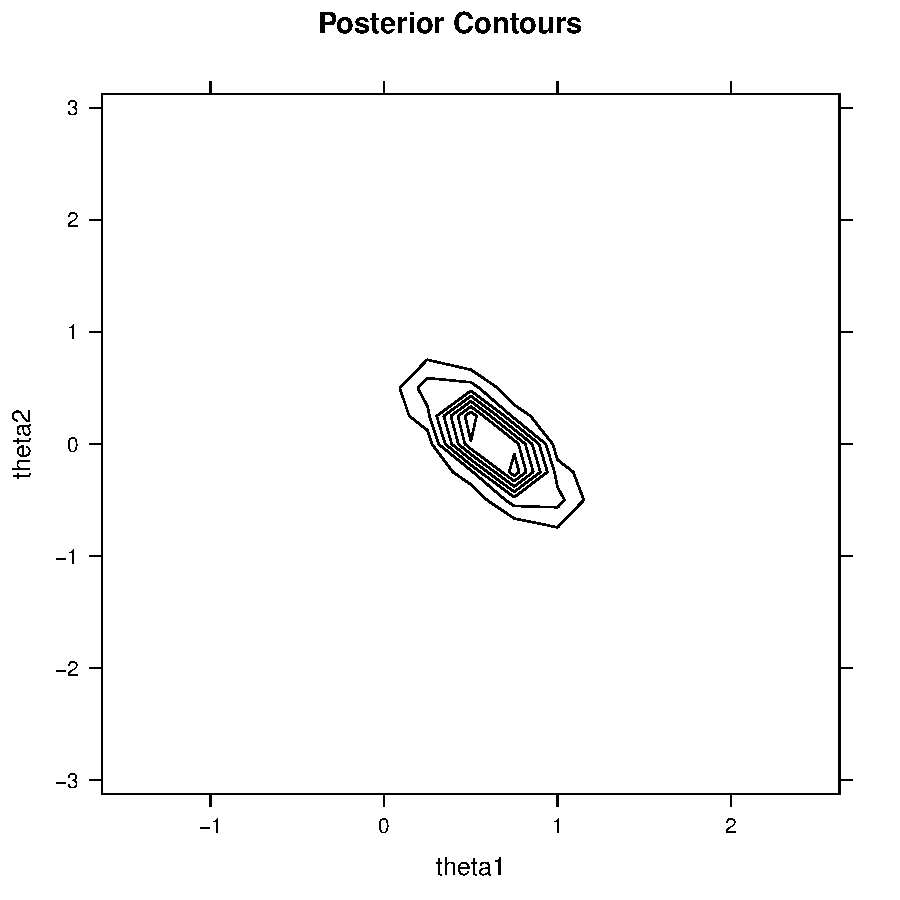
\includegraphics[scale=0.5]{fig1left.pdf}
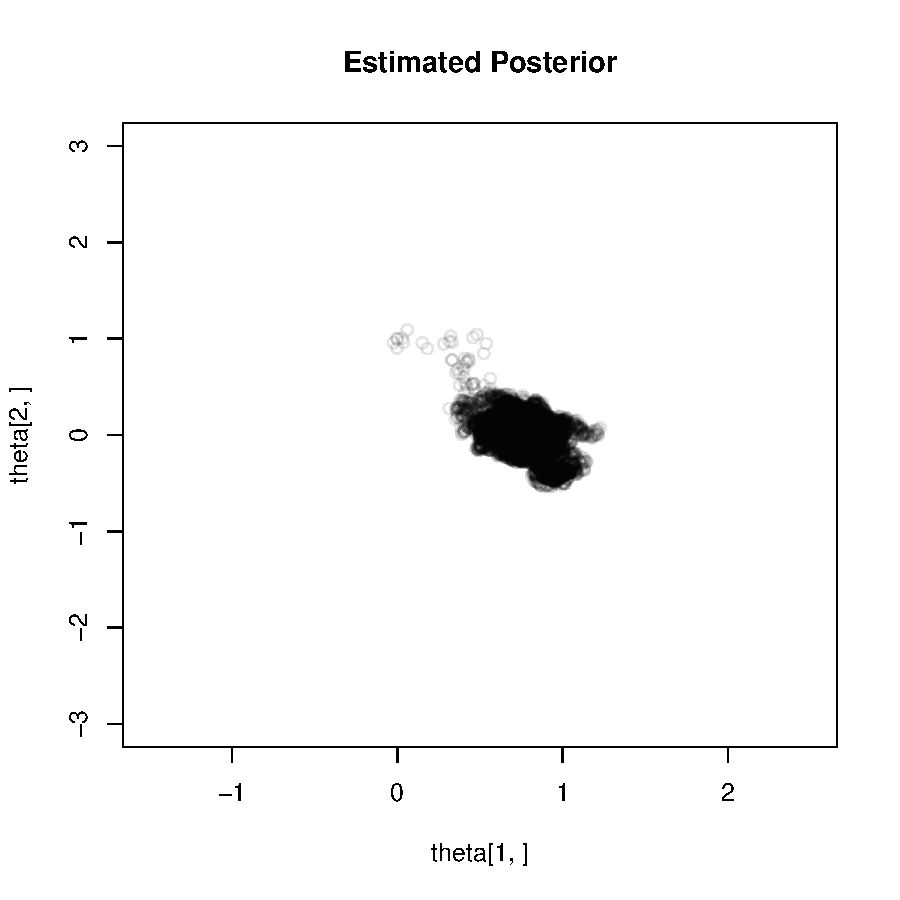
\includegraphics[scale=0.5]{fig1right.pdf}
\end{center}
Judging from the plots of the contours and the estimated posteriors, we see that they are similar to what is given in the paper, but they are more round. It appears that the sampling algorithm stays around only one of the modes $\theta_1 = 0, \theta_2 = 1$ as opposed to going between the other one as well (at $\theta_1 = 1, \theta_2 = -1$).
\begin{center}
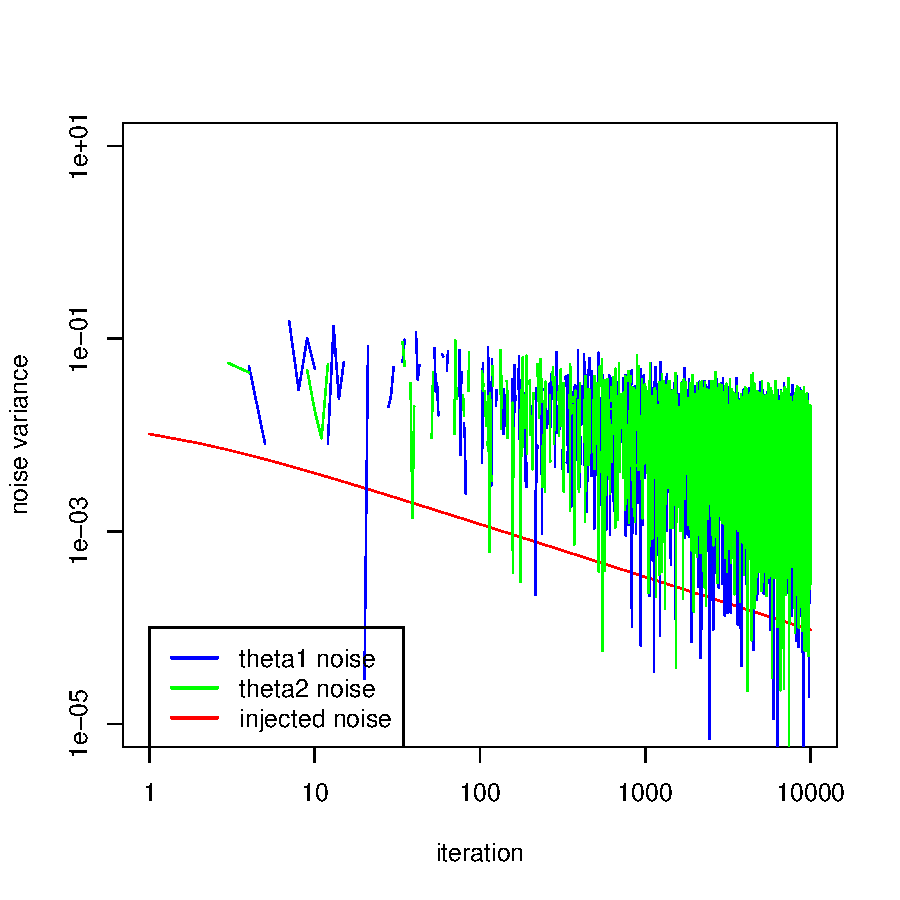
\includegraphics[scale=0.5]{fig2left.pdf}
\end{center}
This plot is again, similar to the one in the paper, however it appears as if the $\nabla \theta_1$ noise and $\nabla \theta_2$ noise plots are much thicker. Secondly, it does not go go below the injected noise as it does in the paper. However, note that there are only 10000 iterations here as opposed to the 100000 in the paper.\\

\noindent
\textbf{Code:}

\begin{verbatimcode}
sigma = c(sqrt(10),1)
sigma.x = sqrt(2)

theta = matrix(c(0,1),nrow=2,ncol=1)
# theta = matrix(c(1,-1),nrow=2,ncol=1)
eta = matrix(,nrow=2,ncol=0)

x = 1/2*rnorm(100, mean=theta[1,1], sd=sigma.x) +
  1/2*rnorm(100, mean=theta[1,1] + theta[2,1], sd = sigma.x)

N=length(x)
n=1

time = 1:10000
a = 0.015
b = 1
gamma = 0.55


epsilon = a*(b+time)^(-gamma)
epsilon[1]
epsilon[length(epsilon)]

t=1
for(t in 1:10000)
{
  #set most recent theta as previous theta
  theta.old = theta[,ncol(theta)]
  #gradient of the log of the prior
  logprior.grad = -theta.old/sigma
  #gradient of the loglikelihood
  ll.grad = function(xtemp)
  {
    const = 1/(exp(-(xtemp-theta.old[1])^2/(2*sigma.x^2)) +
         exp(-(xtemp-theta.old[1]-theta.old[2])^2/(2*sigma.x^2)))
    vec = c()
    vec[1] = exp(-(xtemp - theta.old[1])^2/(2*sigma.x^2)) * (xtemp - theta.old[1])/sigma.x^2 +
      exp(-(xtemp - theta.old[1] - theta.old[2])^2/(2*sigma.x^2)) * (xtemp - theta.old[1] - theta.old[2])/sigma.x^2
    vec[2] = exp(-(xtemp - theta.old[1] - theta.old[2])^2/(2*sigma.x^2)) *
      (xtemp - theta.old[1] - theta.old[2])/sigma.x^2
    const*vec
  }

  eta = cbind(eta,rnorm(2,mean=0,sd=sqrt(epsilon[t])))
  ll.grad.vec = sapply(x[1:n],ll.grad)

  #proposed update
  theta.new = theta.old + epsilon[t]/2*(logprior.grad + N/n*apply(ll.grad.vec,1,sum)) + eta[,ncol(eta)]
  theta = cbind(theta,theta.new)
  theta.old = theta.new
}

plot(theta[1,],theta[2,],xlim=range(-1.5,2.5),ylim=range(-3,3))

pdf("fig1right.pdf",width=6,height=6)
plot(theta[1,],theta[2,],xlim=range(-1.5,2.5),ylim=range(-3,3),col=rgb(0,0,0,alpha=0.1),main="Estimated Posterior")
dev.off()

# plot(c(),xlim=range(-1.5,2.5),ylim=range(-3,3))
# text(theta[1,],theta[2,],labels=c(1:10000))



#Contours of Posterior
library(lattice)
prior = function(theta1,theta2){dnorm(theta1,mean=0,sd=sigma[1])*dnorm(theta2,mean=0,sd=sigma[2])}
likelihood = function(x,theta1,theta2)
{
  1/2*dnorm(x,mean=theta1,sd=sigma.x) + 1/2*dnorm(x,mean=theta1+theta2,sd=sigma.x)
}
C = 0
for(theta1 in seq(-5,5,by=0.25))
{
  for(theta2 in seq(-5,5, by=0.25))
  {
    total_likelihood = 1
    for(i in 1:length(x))
      total_likelihood = total_likelihood * likelihood(x[i],theta1,theta2)
    C = C + prior(theta1, theta2) * total_likelihood
  }
}
C
posterior = function(theta1,theta2,x)
{
  post = prior(theta1,theta2)
  for(i in 1:length(x))
    post = post * likelihood(x[i],theta1,theta2)
  post/C
}

#check if constant works
final_likelihood = 0
posts = c()
for(theta1 in seq(-5,5,by=0.25))
{
  for(theta2 in seq(-5,5, by=0.25))
  {
    final_likelihood = final_likelihood + posterior(theta1, theta2, x)
    posts = c(posts,posterior(theta1, theta2, x))
  }
}
final_likelihood



theta1 = seq(-1.5,2.5,0.25)
theta2 = seq(-3,3,0.25)
ab.grid = expand.grid(theta1=theta1,theta2=theta2)
z = matrix(nrow=length(theta1),ncol=length(theta2))
for(i in 1:length(theta1))
  for(j in 1:length(theta2))
    z[i,j] = posterior(theta1[i],theta2[j],x)
ab.grid$z = c(z)

#Figure 1
pdf("fig1left.pdf",width=6,height=6)
print(contourplot(z ~ theta1*theta2, data=ab.grid, cuts=8, labels=FALSE,main="Posterior Contours"))
dev.off()

#Figure 2
pdf("fig2left.pdf",width=6,height=6)
plot(epsilon,type='l',log="xy",ylim=range(10e-6,10e0),col="red",xlab="iteration",ylab="noise variance")
lines(diff(theta[1,]),col="blue")
lines(diff(theta[2,]),col="green")
legend(1,0.0001,c("theta1 noise","theta2 noise","injected noise"),col=c("blue","green","red"),lwd=c("2","2","2"))
dev.off()
\end{verbatimcode}
\begin{comment}$\end{comment}

\item 
In this section, we look at the \texttt{a9a} dataset from the UCI \texttt{adult} dataset, consisting of 32561 observations and 123 features. We have outputs $y_i \in \{-1, +1\}$ given corresponding input vectors $x_i$. They are modeled as 
\[\p{y_i | x_i} = \frac{\exp(y_i \beta' x_i)}{1 + \exp(y_i \beta' x_i)}\]
This is slightly different from the standard logistic regression (where we have 0's and 1's as responses). However, we have that
\begin{align*}
\p{y_i = 1 | x_i} &= \frac{\exp(\beta' x_i)}{1 + \exp(\beta' x_i)}\\
\p{y_i = -1 | x_i} &= \frac{\exp(-\beta' x_i)}{1 + \exp(-\beta' x_i)}\\&= \frac{1}{1 + \exp(\beta' x_i)}
\end{align*}
and so
\[\p{y_i = 1 | x_i} + \p{y_i = -1 | x_i} = 1\]

Using a Laplace prior on $\beta$ with scale 1, we have
\[\p{\beta} = \frac{1}{2} e^{-|\beta|}\]
Taking logs, we get
\[\log \p{\beta} = \log\left(\frac{1}{2}\right) - |\beta|\]
Finally, differentiating with respect to $\beta$ gives us
\[\nabla \log \p{\beta} = -\sgn(\beta)\]

if we take the log of our likelihod, which is given above, we get
\begin{align*}
\log \p{y_i | x_i} &= \log \exp(y_i \beta' x_i) - \log (1 + \exp(y_i \beta' x_i))\\
&= y_i \beta' x_i - \log (1 + \exp(y_i \beta' x_i))
\end{align*}
Differentiating this with respect to $\beta$ gives
\begin{align*}
\frac{\partial}{\partial \beta} \log \p{y_i | x_i} &= y_i x_i - \frac{\exp(y_i \beta' x_i)}{1 + \exp(y_i \beta' x_i)} y_i x_i\\
&= \frac{y_i x_i}{1 + \exp(y_i \beta' x_i)}
\end{align*}
Using these two gradients, we can form our stochastic gradient Langevin algorithm as follows: At each iteration $t$, we have
\begin{align*}
\beta_{t+1} &= \beta_t + \frac{\varepsilon_t}{2}\left\{\nabla \log \p{\beta_t} + \frac{N}{n} \sumin \nabla \log \p{y_{ti} | x_i, \beta_t} \right\} + \eta_t\\
&= \beta_t + \frac{\varepsilon_t}{2}\left\{-\sgn(\beta) + \frac{N}{n} \sumin \frac{y_i x_i}{1 + \exp(y_i \beta' x_i)}\right\} + \eta_t
\end{align*}
where $\sgn(\beta)$ is the sign function applied termwise to each coordinate of $\beta$. The $\eta_t$ term is our noise term where $\eta_t \sim \sN(0, \varepsilon_t)$.

\begin{center}
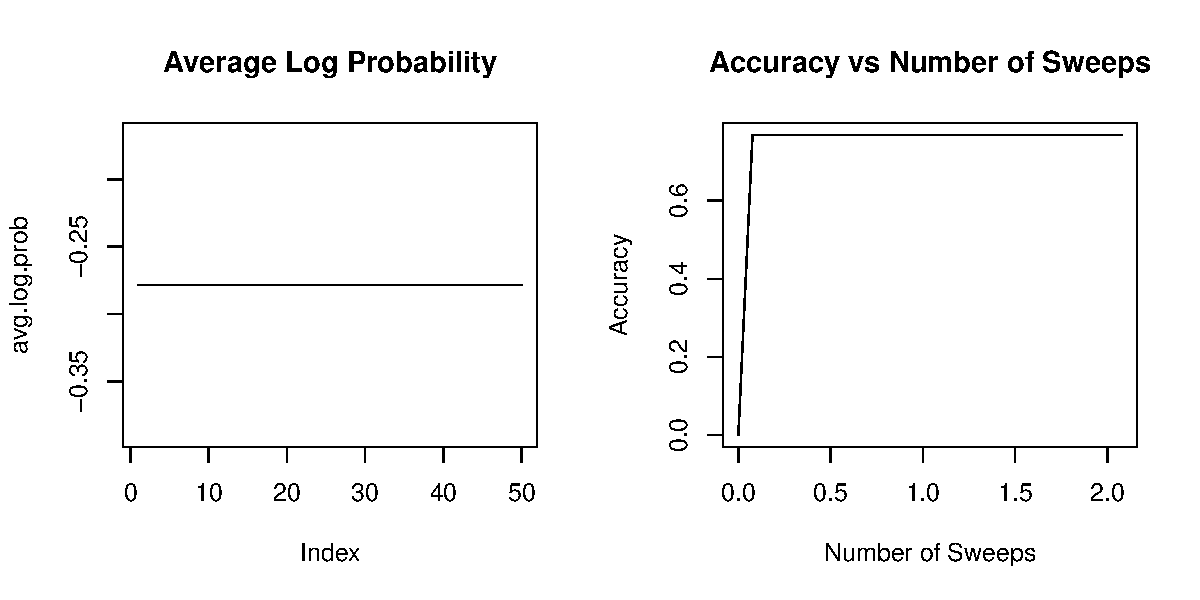
\includegraphics[scale=0.5]{fig3.pdf}
\end{center}
We can see that it achieves convergence of both the log joint probability and the accuracy very quickly.\\

\noindent
\textbf{Code:}
\begin{verbatimcode}
data = read.csv("a9a",sep=" ",header=FALSE)
data = data[,-16] #removes last column which is glitchy (all NA)

x = matrix(,nrow=32561,ncol=14)

for(cols in 1:14)
{
  #Extracts the number x from the string "x:1"
  x[,cols] = sapply(as.character(data[,cols+1]), function(i) as.numeric(strsplit(i,":")[[1]][1]))
}
y = data[,1]

#Split x and y into training and test sets
train.indices = sample(1:nrow(x),0.8*nrow(x))
x.train = x[train.indices,]
x.test = x[-train.indices,]
y.train = y[train.indices]
y.test = y[-train.indices]

#Creates design matrix from the matrix of indices x.train
x.mat.train = matrix(0,nrow=nrow(x.train), ncol=123)
for(i in 1:nrow(x.mat.train))
  x.mat.train[i,x.train[i,]]=1
x.mat.train = cbind(1,x.mat.train)

x.mat.test = matrix(0,nrow=nrow(x.test), ncol=123)
for(i in 1:nrow(x.mat.test))
  x.mat.test[i,x.test[i,]]=1
x.mat.test = cbind(1,x.mat.test)


#Set Parameters
N = nrow(x)
n = 10

time = 1:50
a = 0.015
b = 1
gamma = 0.55

epsilon = a*(b+time)^(-gamma)
epsilon[1]
epsilon[length(epsilon)]

expit = function(x){1/(1+exp(-x))}
beta.mat = matrix(0,nrow=124,ncol=1)

for(t in 1:50)
{
  for(batch.rep in seq(1,124,10))
  {
    n=10
    if(batch.rep==121)
      n=4
    beta.old = beta.mat[,ncol(beta.mat)]
    logprior.grad = sign(beta.old)
    ll.grad = function(index)
    {
      expit(y.train[index] * sum(beta.old * x.mat.train[index,])) * y.train[index] * x.mat.train[index,]
    }

    eta = rnorm(124,mean=0,sd=sqrt(epsilon[t]))
    ll.grad.vec = sapply(1:n,ll.grad)

    #proposed update
    beta.new = beta.old + epsilon[t]/2*(logprior.grad + N/n*apply(ll.grad.vec,1,sum)) + eta
    beta.mat = cbind(beta.mat,beta.new)
    beta.old = beta.new
  }
}

length(y.train)
dim(x.mat.train)
dim(beta.mat)

#indices when entire sweep of dataset has finished
beta.index = seq(14,13*50+1,13)
beta.final = beta.mat[,beta.index]

#Average log joint probability per data item vs number of sweeps
avg.log.prob = c()
for(i in 1:ncol(beta.final))
{
  temp = mean(expit(y.train * x.mat.train %*% beta.final[,i]))
  avg.log.prob = c(avg.log.prob, log(temp))
}

pdf("avglogprob.pdf",weight=6,height=6)
dev.off()


#Accuracy on test set vs number of swepes
length(y.test)
dim(x.mat.test)
dim(beta.mat)

#vector of accuracies
acc = c()
for(i in 1:ncol(beta.mat))
{
  probs = expit(y.test * x.mat.test %*% beta.mat[,i])
  temp = length(which(probs>0.5))/length(probs)
  acc = c(acc,temp)
}
pdf("fig3.pdf",width=8,height=4)
par(mfrow=c(1,2))
plot(avg.log.prob,type='l',main="Average Log Probability")
plot((1:28-1)/13, acc[1:28],type='l',xlab="Number of Sweeps",ylab="Accuracy",main="Accuracy vs Number of Sweeps")
dev.off()
\end{verbatimcode}



\item 
In this part, we use the SGLD method to sample from the banana-shaped posterior in the Raftery model which was done in problem set 4. The model is set up as follows: our prior is of the form
\[\p{N, \theta} \propto \frac{1}{N} \mathds{1}_{\theta \in [0,1]}\]
and our likelihood is a Binomial.
\[\p{Y_1,\ldots,Y_n | N, \theta} = \prodin \binom{N}{y_i} \theta^{y_i} (1-\theta)^{N-y_i} \]
Using these, we wish to sample from $N,\theta | Y_1,\ldots,Y_n$.

Ideally, we would use the stochastic gradient Langevin dynamics method on both the $\theta$ and $N$ parameters, but difficulties arise as we cannot differentiate with respect to $N$ because it is a discrete parameter. Instead, at each iteration, we generate $N_t$ as in problem set 4, where we take 
\[N_{t+1} \sim \Geom\left(\frac{1}{1 + N_t}\right)\]
This way, we have that $\E{N_{t+1}} = N_t$. Now, based on the above prior and likelihood, we can derive the appropriate gradients. First, we will look at the prior. Taking the log, we get
\[\log \p{N_t, \theta_t} = - \log(N_t) \mathds{1}_{\theta_t \in [0,1]} \]
Then differentiating with respect to $\theta_t$, we get
\begin{equation}\label{priorderiv}
\frac{\partial}{\partial \theta_t} \log \p{N_t, \theta_t} = - \log (N_t)\mathds{1}_{\theta_t \in [0,1]}
\end{equation}
Now, we look at the likelihood. Taking the log, we get that the log-likelihood is 
\[\log \p{Y_1,\ldots,Y_n | N_t, \theta_t} = \sumin y_i \log (\theta_t) + (N_t - y_i) \log(1-\theta_t) + \log \binom{N_t}{y_i}\]
Differentiating with respect to $\theta_t$ gives
\begin{equation}
\frac{\partial}{\partial \theta_t} \log \p{Y_1,\ldots,Y_n | N_t, \theta_t} = \sumin \frac{y_i}{\theta_t} - \frac{N_t - y_i}{1-\theta_t}
\end{equation}\label{likelihoodderiv}

Using these, use the stochastic gradient Langevin dynamics method as described by Welling and Teh, with the iterative steps defined as
\begin{align*}
\theta_{t+1} &= \theta_t + \frac{\varepsilon_t}{2}\left(\nabla \log \p{N_t, \theta_t} + \frac{N}{n} \sumin \nabla \log \p{y_{ti} | N_t, \theta_t} \right) + \eta_t\\
&= \theta_t + \frac{\varepsilon_t}{2}\left(\nabla \log \p{N_t, \theta_t} + \sum_{i=1}^N \nabla \log \p{y_{ti} | N_t, \theta_t} \right) + \eta_t\\
&= \theta_t + \frac{\varepsilon_t}{2}\left\{-\log(N_t)\mathds{1}_{\theta_t \in [0,1]} + \sum_{i=1}^N \left( \frac{y_i}{\theta_t} - \frac{N_t - y_i}{1 - \theta_t} \right) \right\}+ \eta_t
\end{align*}
where $\varepsilon_t$ are our carefully chosen step sizes and $\eta_t \sim \sN(0, \eta_t)$ is injected noise for our Langevin dynamics. The gradients $\nabla \log \p{N_t, \theta_t}$ and $ \nabla \log \p{y_{ti} | N_t, \theta_t}$ are the same derivatives calculated above in equations \eqref{priorderiv} and \eqref{likelihoodderiv} since $\theta_t$ is univariate. Note that we set $n=N$, so that $\frac{N}{n}=1$. As $N=5$, we do not need to use a mini-batch of our data because it is already small enough for us to computation over the entire dataset without sacrificing too much computation time.

The algorithm operates as follows: First, we define
\[\varepsilon_t = a(b + t)^{-\gamma}\]
as before. We initialize $N_0=\max(y)$ and $\theta_0=0.9$. At iteration $t$, we sample
\[N_{t+1} \sim \Geom\left(\frac{1}{1+N_t}\right)\]

\begin{framed}
\begin{algorithmic}
\State $N_0 = \max(y)$
\State $\theta_0 = 0.9$
\For {$t=1,2,\ldots$}
\State $\varepsilon_t = a(b+t)^{-\gamma}$
\State $\eta_t \sim \sN(0, \varepsilon_t)$
\State $N_{t+1} \sim \Geom\left(\frac{1}{1 + N_t}\right)$
\State $\theta_{t+1} = \theta_t + \frac{\varepsilon_t}{2}\left(\nabla \log \p{N_t, \theta_t} + \sum_{i=1}^N \nabla \log \p{y_{ti} | N_t, \theta_t}\right) + \eta_t$
\If {$\theta_{t+1} \geq 1$}
\State $\theta_{t+1} = 1 - 10^{-6}$
\EndIf
\If {$\theta_{t+1} \leq 0$}
\State $\theta_{t+1} = 10^{-6}$
\EndIf
\EndFor
\end{algorithmic}
\end{framed}

Note that if $\theta_{t+1} > 1$ or $\theta_{t+1} < 0$, we need to move back into the unit interval since we require that $0 \leq \theta_{t+1} \leq 1$ as $\theta_{t+1}$ is a probability. However, if we set them back to 1 or 0 respectively that would create a division by 0 in the $\nabla \log \p{y_{ti} | N_t, \theta_t}$ term. Instead, by adding/subtracting a tiny amount off of it, it ensures we have a valid gradient.

The choice of the learning rate, which depends on $a$,$b$, and $\gamma$, is very important as these values determine the convergence properties of the algorithm.

Results for waterbuck:
\begin{center}
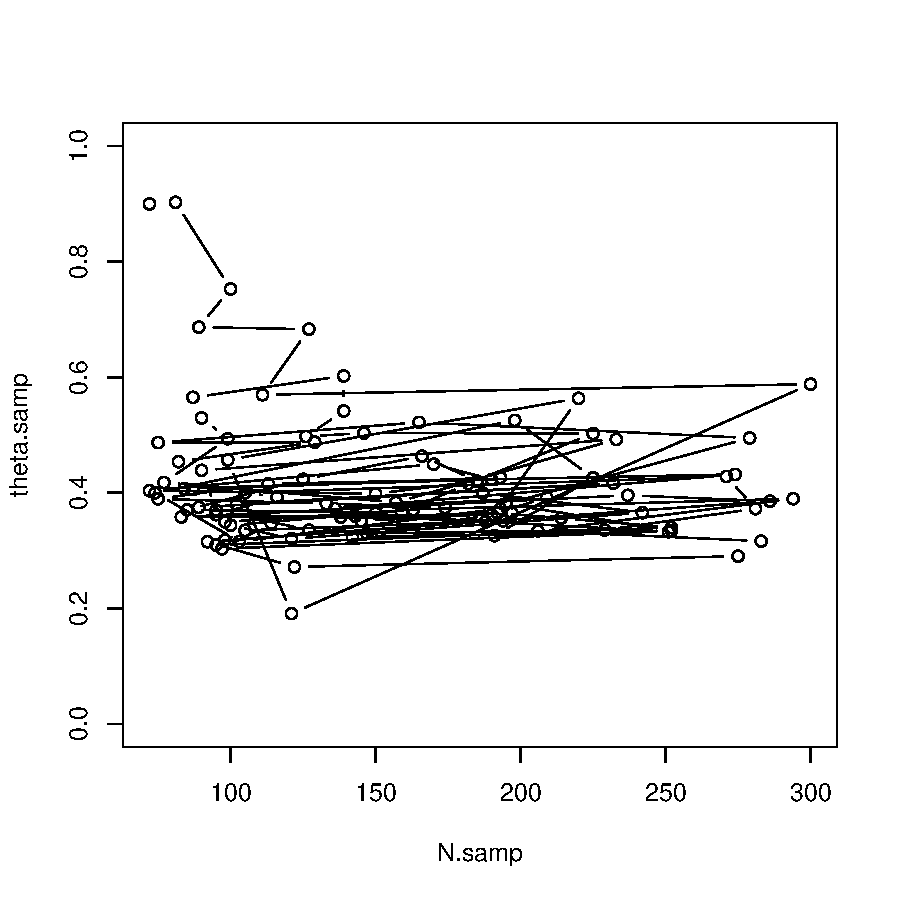
\includegraphics[scale=0.5]{waterbuck-scatterplot.pdf}
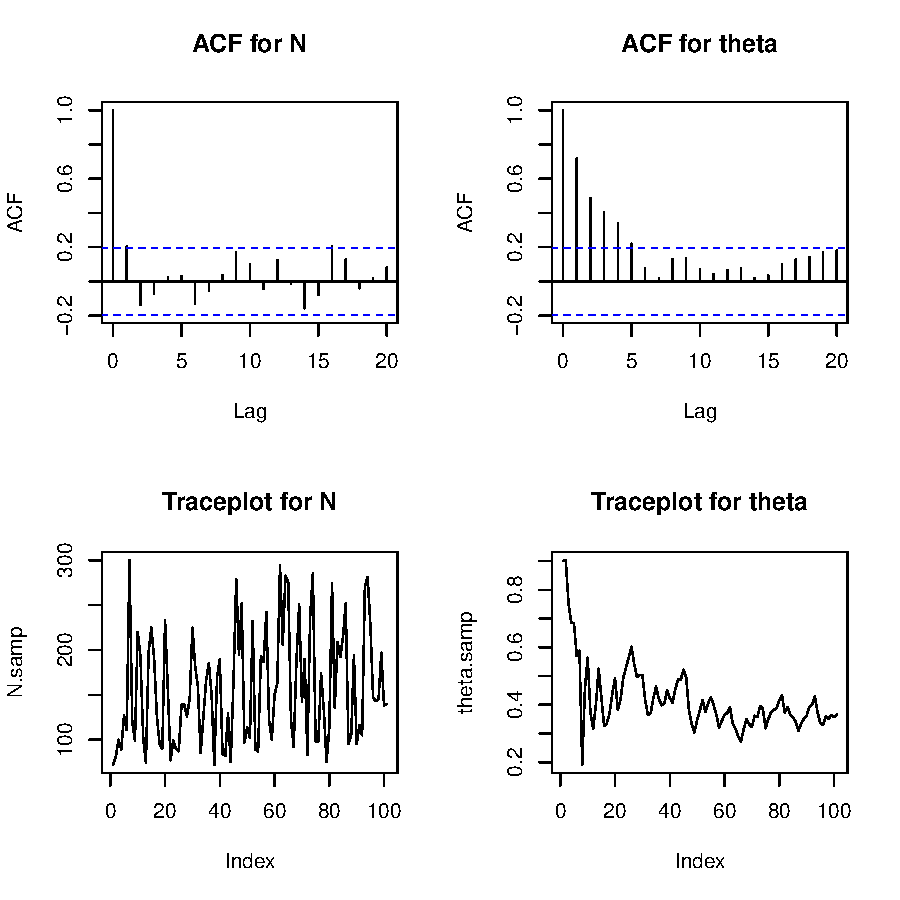
\includegraphics[scale=0.5]{waterbuck-diagnostics.pdf}
\end{center}

Results for impala:
\begin{center}
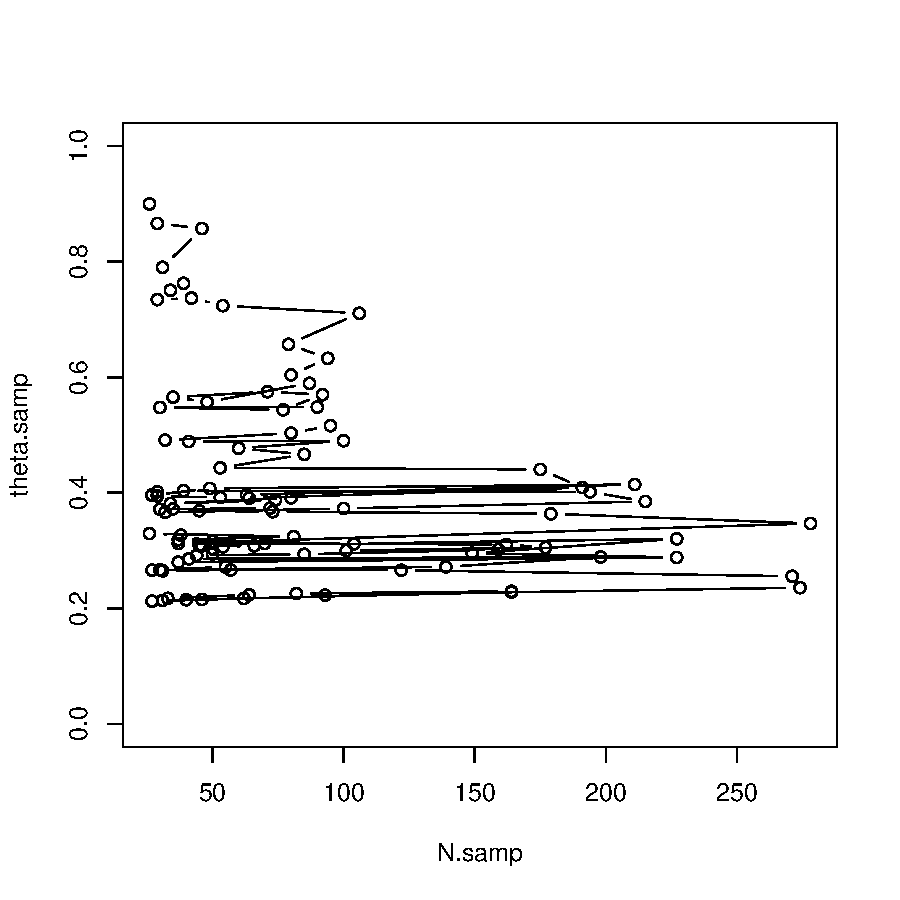
\includegraphics[scale=0.5]{impala-scatterplot.pdf}
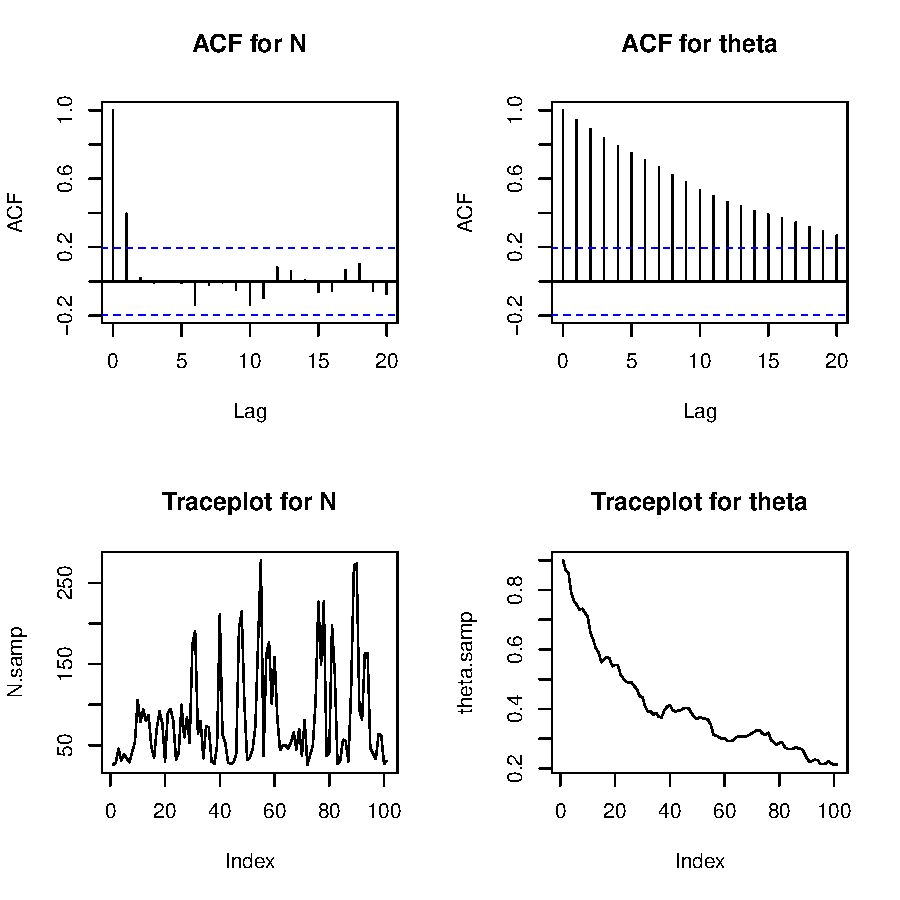
\includegraphics[scale=0.5]{impala-diagnostics.pdf}
\end{center}

We see that in the scatterplots for both the impala and waterbuck we have the rough banana shaped posterior we desire. However, looking at the traceplots and ACF plots for $\theta$, we see that this is not the best. One important observation is that the $\theta$ seems to descend slowly from 1 to 0 and the randomness of the $N$ fills out the shape of the posterior. If the chain were to keep running, it appears that if would stay in the bottom flat portion of the distribution and never return to the vertical part. In particular, looking at the traceplot for $\theta$ in waterbuck, we see that once it goes through its initial descent, $\theta$ has a more regular traceplot with less autocorrelation.\\


\noindent
\textbf{Code:}
\begin{verbatimcode}
impala = read.table("impala.txt", header = TRUE)
impala = impala[,1]

waterbuck = read.table("waterbuck.txt", header = TRUE)
waterbuck = waterbuck[,1]

log.lik <- function(Y, N, theta)
{
  # Log-likelihood of the data
  sum(dbinom(Y, N, theta, log=T))
}

log.prior <- function(N, theta)
{
  #1/N times the indicator that theta is in [0,1]
  log(1/N * ifelse(theta>=0 & theta<=1,1,0))
}

time = 1:1000

#impala
a = 0.0005
b = 3
gamma = 0.7

#waterbuck
a = 0.002
b = 5
gamma = 0.7

epsilon = a*(b+time)^(-gamma)
epsilon[1]
epsilon[length(epsilon)]

y = impala
y = waterbuck
S = sum(y)
theta.samp = 0.9
N.samp = max(y)

for(t in 1:100)
{
  theta.old = tail(theta.samp,1)
  N.old = tail(N.samp,1)

  #ensures N is large enough
  repeat
  {
    #geometric over entire thing
    N.new = rgeom(1,1/(1+N.old))
    #only keep sample if N is in the boundaries
    if(N.new >= max(y) & N.new <= 300)
      break
  }

  logprior.grad = -log(N.old)
  ll.grad = function(index)
  {
    y[index]/theta.old - (N.old - y[index])/(1-theta.old)
  }

  ll.grad.vec = sapply(1:5,ll.grad)
  eta = rnorm(1,mean=0,sd=sqrt(epsilon[t]))

  #proposed update
  theta.new = theta.old + epsilon[t]/2*(logprior.grad + sum(ll.grad.vec)) + eta
  #if theta.new is outside boundaries, project back to [0,1]
  #theta.new cannot be 0 or 1 otherwise ll.grad becomes infinite
  #so we add a bit of noise
  if(theta.new>1)
    theta.new=1-1e-6
  if(theta.new<0)
    theta.new=1e-6

  #Add theta to samples
  theta.samp = c(theta.samp,theta.new)
  theta.old = theta.new
  #Add N to samples
  N.samp = c(N.samp,N.new)
  N.old = N.new
}

N.samp
theta.samp



pdf("waterbuck-scatterplot.pdf",width=6,height=6)
plot(N.samp,theta.samp,type="b",ylim=range(0,1))
dev.off()


pdf("waterbuck-diagnostics.pdf",width=6,height=6)
par(mfrow=c(2,2))
acf(N.samp, main="ACF for N")
acf(theta.samp, main="ACF for theta")
plot(N.samp,type='l',main="Traceplot for N")
plot(theta.samp,type='l',main="Traceplot for theta")
dev.off()


pdf("impala-scatterplot.pdf",width=6,height=6)
plot(N.samp,theta.samp,type="b",ylim=range(0,1))
dev.off()


pdf("impala-diagnostics.pdf",width=6,height=6)
par(mfrow=c(2,2))
acf(N.samp, main="ACF for N")
acf(theta.samp, main="ACF for theta")
plot(N.samp,type='l',main="Traceplot for N")
plot(theta.samp,type='l',main="Traceplot for theta")
dev.off()
\end{verbatimcode}

\end{enumerate}


\section{Conclusion}
The stochastic gradient Langevin dynamics method is a combination of stochastic gradient descent and Langevin dynamics in order to sample from a posterior distribution. On its own, the stochastic gradient descent algorithm leads to the MAP (maximum a posteriori) value, therefore encouraging the algorithm to spend more time in high probability areas. Langevin dynamics adds noise to each iteration to perturb it so it does not collapse onto the MAP value, but rather hovers around it. This allows it to explore to entire parameter space. 

Choice of the parameters, namely how $\varepsilon_t$ is formulated, is very important. This variance parameter influences the fluidity of the MCMC chain. If the variance is too small, it will not move at all. If it is too large, it will only take the values 0 or 1.

Another issue that arose in the sampling was the constraints that were put on $\theta$. If $\theta$ lay outside the $[0,1]$ interval, we simply projected back into it (that is, set it to $10^{-6}$ or $1-10^{-6}$ respectively). Perhaps an alternative, more ideal solution would be to reparameterize the $\theta$ parameter to something which lives on the reals, so that we can never exit the parameter space. An obvious example is to use the expit function that is used in a logistic regression
\[y = \frac{\exp(\theta)}{1 + \exp(\theta)}\]
Another suitable candidate would be the inverse probit function
\[y = \Phi^{-1}(\theta)\]
However, if we were to do a transformation, there is the caveat that we would need to rederive the gradients as we would be differentiating with respect to something else.








\end{document}

